\begin{justifying}
    \begin{center}
        CAPÍTULO 5
    \end{center}
    
    \begin{center}
        4. ACCIÓN Y REACCIÓN
    \end{center}

    4.1. Cambio inducido
    Hasta ahora nos hemos ocupado del cambio sin tener en cuenta sus
    orígenes. Ahora bien, una cosa puede cambiar por sí misma o bajo la influencia
    de otra cosa, es decir, espontáneamente o por inducción. Por lo tanto, debemos
    estudiar los conceptos de espontaneidad e inducción. Para ello,
    nos valeremos del concepto de historia (Definición 5.27 en la Sec.
    3.2) y de la ley de Leibniz (Cap. 2, Sec. 3.2).
    Dos cosas diferentes del mismo tipo pueden describirse con la ayuda
    del mismo esquema funcional (M, IF), por lo tanto, del mismo espacio de estados,
    aunque, por supuesto, añadiendo circunstancias individualizadoras en cada caso. En
    otras palabras, los estados de cosas diferentes del mismo tipo pueden representarse en
    un mismo espacio de estados. Además, cada espacio de estados, lejos de ser
    propiedad de una sola cosa, puede asignarse a una clase de referencia constituida por
    una clase de equivalencia más o menos numerosa de cosas. Ahora bien, la ley de Leibniz
    (Postulado 2.5 o Corolario 2.1) establece que cosas diferentes tienen propiedades diferentes.
    Por lo tanto, incluso si una función de estado dada describe adecuadamente
    dos cosas, estas no pueden ocupar exactamente los mismos estados, ya que, si lo hicieran,
    serían una sola. En consecuencia, tenemos la siguiente reformulación de
    la ley de Leibniz: 

    COROLARIO 5.11 Las cosas diferentes tienen historias diferentes.
    Sin duda, una cosa puede ocupar ahora exactamente el mismo estado en el que se encontraba otra cosa
    hace un momento, pero no hay dos cosas que puedan ocupar exactamente el mismo
    estado al mismo tiempo o, más en general, para el mismo valor del
    parámetro de cambio. (Véase la figura 5.14). 

    \begin{figure}[h!]
    \centering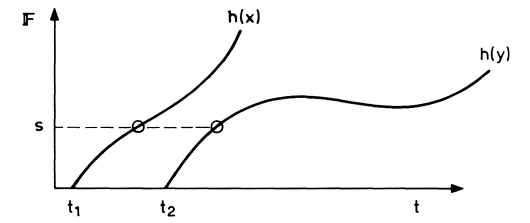
\includegraphics[width=0.6\textwidth]{img/grafico5.14.png}
    \caption{\label{fig:espacio_estados} Fig. 5.14. Diferentes cosas pueden ocupar el mismo estado siempre que lo hagan en
    momentos diferentes.}
    \end{figure}

    \pagebreak

    \begin{center}
        CAMBIO
    \end{center}

    El corolario 5.11 es nuestra versión actual del princlplum
    individuationis de Leibniz y nos da la clave de lo que buscamos. De hecho, si una
    cosa está bajo la acción de otra cosa, entonces su historia debe diferir
    de la historia cuando está libre de dicha acción. (Véase la figura 5.15). (En esto
    consiste el experimento científico, a diferencia de la observación,
    es decir, en activar y desactivar deliberadamente acciones o influencias para
    comparar el comportamiento forzado de una cosa con su comportamiento libre y así
    evaluar la importancia de la variable que se está manipulando).

    \begin{figure}[h!]
    \centering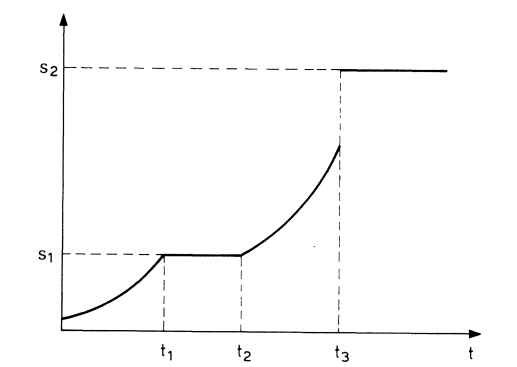
\includegraphics[width=0.6\textwidth]{img/grafico5.15.png}
    \caption{\label{fig:grafico_5_15} Fig. 5.15. [Fig. 5.15. Ejemplo imaginario de una acción. El agente, al actuar durante el intervalo [f1, t2],
    obliga al paciente a permanecer en el estado 51'. La acción externa se reanuda en el momento f3,
    obligando al paciente a saltar al estado 52'. ].}
    \end{figure}

    En ausencia de cualquier acción del agente x sobre el paciente y, la
    historia de su suma física o yuxtaposición x + y es igual a la unión de
    sus líneas de comportamiento individuales. En otras palabras, tenemos

    DEFINICIÓN 5.28 La cosa x cambia por sí misma, o espontáneamente, si y solo si h(x) no es
    un singleton y, para cualquier otra cosa y

    \begin{center}
        $h(x \dot{+} y) = h(x) \cup h(y)$.
    \end{center}
    
    Claramente, si una de las cosas actúa sobre la otra, entonces, mientras que la
    línea de comportamiento del agente permanece inalterada, la del paciente 

    \pagebreak

    \begin{center}
        CAPÍTULO 5
    \end{center}

    se convierte, por así decirlo, en la historia de otra cosa a saber,
    la cosa sobre la que actúa el agente. (Véase la figura 5.16.) Más exactamente, hacemos

    \begin{figure}[h!]
    \centering
    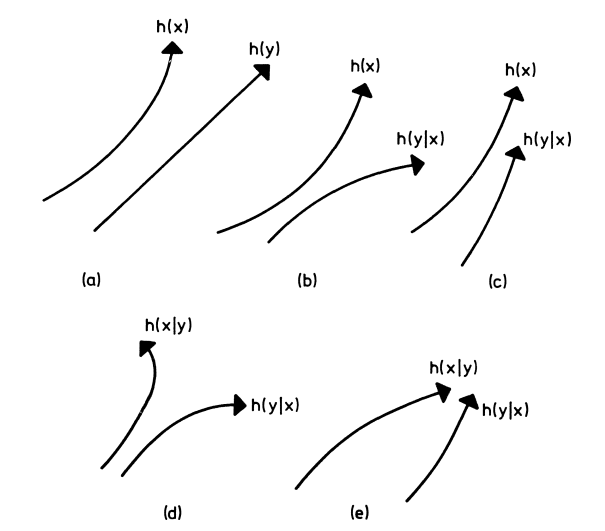
\includegraphics[width=0.6\textwidth]{img/grafico5.16.png}
    \caption{\label{fig:grafico_5_16} Fig. 5.16. [Cambio inducido. (a) Sin acción: cambio espontáneo tanto de x como de y.
    (b) Acción de empuje de x sobre y. (c) Acción de tracción de x sobre y. (d) Interacción de empuje.
    (e) Interacción de tracción. ].}
    \end{figure}

    DEFINICIÓN 5.29 Sean X e y dos cosas diferentes con funciones de estado IF y G respectivamente relativas a un marco de referencia común t, y 
    sea
    
    \begin{center}
        $$ h(y|x) = \{ \langle t, \mathbb{H}(t) \rangle | t \in S(f) \} $$.
    \end{center}

    serán sus respectivas historias. Además, sea IHI = g(lF, G) ¢ G una tercera función de estado,
    dependiente tanto de IF como de G, y llamemos

    \begin{center}
        $$ h(x) = \{ \langle t, F(t) \rangle | t \in S(f) \}, \quad h(y) = \{ \langle t, G(t) \rangle | t \in S(f) \} $$.
    \end{center}

    La historia correspondiente. Entonces x actúa sobre y, o x [> y para abreviar, si y solo si, para
    alguna función de estado IHI que determina la trayectoria h (y Ix),
    h (y Ix) ¢ h (y ). 

    \pagebreak

    \begin{center}
        CAMBIO
    \end{center}

    Ahora podemos reformular la definición 5.28 de espontaneidad: Una cosa
    cambia espontáneamente si y solo si cambia y no hay ninguna otra cosa que
    actúe sobre ella. Y, a partir de la hipótesis de la definición 5.29 (en particular,
    que x '¢ y), se deduce que nada actúa sobre sí mismo.
    La definición de acción recíproca o mutua es ahora obvia:

    DEFINICIÓN 5.30 Dos cosas diferentes x e y interactúan si y solo si cada una actúa sobre
    la otra. En símbolos:

    \begin{center}
        $$ x \bowtie y =_{\text{df}} x \rhd y \ \& \ y \rhd x. $$
    \end{center}

    Los científicos experimentales asumen tácitamente (a) que todas las cosas son estudiables,
    (b) que no hay cosas totalmente aisladas, es decir, que cada cosa actúa sobre otra cosa
    o es afectada por otra cosa, y (c) que tales acciones son la base
    del conocimiento empírico. De hecho, si una cosa supuesta no actúa sobre ninguno
    de nuestros medios de observación, entonces no podemos observarla; y si alguna
    cosa putativa no es afectada por ninguno de nuestros medios experimentales, entonces
    no podemos experimentar con ella. En cualquiera de los dos casos, no nos preocuparemos por «ella». En
    resumen, el siguiente axioma pertenece a la ontología inherente a la ciencia,
    por lo que lo adoptamos:

    POSTULADO 5.10 Todo actúa sobre otras cosas y es afectado por ellas.
    Esta suposición no debe confundirse con la hipótesis mucho más fuerte y
    Esta suposición no debe confundirse con la hipótesis mucho más fuerte, y
    falsa, de que dos cosas cualesquiera interactúan, y mucho menos con la misma
    intensidad. No reaccionamos ante la actividad luminosa del sol, y mucho menos
    ante la de una estrella extinta. En otras palabras, el principio de interacción universal,
    sugerido por primera vez por los estoicos y muy favorecido durante el
    apogeo de la teoría de la gravitación de Newton, es falso.
    Los efectos de una interacción pueden ser duraderos, incluso en el caso de
    las microcosas. Así, si dos microcosas interactúan durante un tiempo y luego dejan
    de hacerlo, por ejemplo, al separarse mucho en el espacio, seguirán
    estando correlacionadas. Por lo tanto, observar una de ellas puede proporcionar
    información sobre la otra, del mismo modo que observar el comportamiento de una
    persona divorciada puede arrojar luz sobre su antigua pareja. En la jerga de la
    mecánica cuántica, se dice que tales cosas son inseparables o que
    muestran una correlación EPR. (Esto es lo que parece ser la paradoja de Einstein-Podolsky-Rosen.
    Más información en la sección 4.2).

    \pagebreak

    Necesitamos un concepto cualitativo del tamaño de una acción o una interacción. Este viene dado por la cantidad de distorsión efectuada por el
    agente o agentes en la línea de comportamiento del paciente. En otras palabras, hacemos
    
    DEFINICIÓN 5.31 Sean x e y dos cosas, y sea h(x) la historia
    de x, y h(xl y) la historia de x cuando actúa sobre y, y de manera similar para
    x. Entonces
    (i) la acción o efecto total de x sobre y es igual a la diferencia entre
    la trayectoria forzada y la trayectoria libre de y:

    \begin{center}
        $$ A(x, y) = h(y|x) \cap \overline{h(y)}; $$.
    \end{center}

    (ii) la reacción total de y sobre x es la diferencia entre la trayectoria libre
    y la trayectoria forzada de x:

    \begin{center}
        $$ A(y, x) = h(x|y) \cap \overline{h(x)}; $$.
    \end{center}

    (iii) la interacción total entre x e y es la unión de acción y
    reacción:

    \begin{center}
        $$ I(x, y) = A(x, y) \cup A(y, x). $$.
    \end{center}

    Si A (x, y) = 0, podemos decir que x ejerce una acción nula sobre y.
    Dado que la acción de x sobre y es un conjunto de eventos en y, este conjunto no puede ser el
    mismo que la reacción de y sobre x, que es un conjunto de eventos en x. Por lo tanto, tenemos
    el

    COROLARIO 5.12 Ninguna acción es igual a la reacción correspondiente. Es decir, para
    cualquier cosa x e y, A(x, y):I= A(y, x).
    Este resultado no es inconsistente con la tercera ley de la mecánica de partículas newtoniana.
    De hecho, esta ley no afirma que las acciones y reacciones sean
    iguales, sino que sus intensidades (las fuerzas correspondientes, o bien
    los pares) son iguales. De todos modos, la ley no se cumple en otras teorías, como
    la electrodinámica.

    Ahora bien, las acciones pueden existir en ciertos aspectos, pero no en otros. Es decir,
    la acción de la cosa x sobre la cosa y puede afectar solo a algunos de los
    componentes de la función de estado de y. Por lo tanto, podemos analizar la acción total
    en acciones parciales, a saber: 

    \begin{center}
        $$ A(x, y) = \bigcup_{i=1}^{m} A_{i}(x, y), $$.
    \end{center}

    \pagebreak

    \begin{center}
        CAMBIO
    \end{center}

    Donde m es el número de acciones mutuamente independientes que x ejerce sobre
    y. Lo mismo ocurre con la reacción de y sobre x y con su interacción.
    Esta distinción nos permite complementar el Postulado 5.8 con

    POSTULADO 1E 5.11 Todo cambia espontáneamente en algunos aspectos,
    y de forma inductiva en otros.
    Por último, el concepto de acción nos permite dilucidar la importante
    distinción que se hace en el capítulo 2, sección 5.1, entre una relación que afecta a sus
    relata y otra que no lo hace. (Véase la figura 5.17.) La diferencia se
    precisa mediante

    DEFINICIÓN 5.32 Dos cosas diferentes están unidas (o vinculadas o
    acopladas) entre sí si y solo si al menos una de ellas actúa sobre la otra. En
    símbolos: si x e y son cosas, entonces

    \begin{center}
        $$ Bxy =_{\text{df}} x \rhd y \ \text{or} \ y \rhd x. $$.
    \end{center}

    Tenga en cuenta que no estamos incluyendo la condición de que el vínculo sea
    atractivo. Dos enemigos están tan unidos como dos amigos.

    \begin{figure}[h!]
    \centering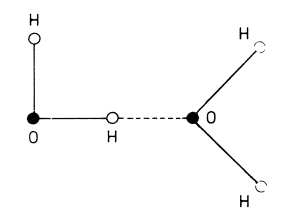
\includegraphics[width=0.6\textwidth]{img/grafico5.17.png}
    \caption{\label{fig:grafico_5_17} Fig. 5.17. [Tres relaciones diferentes entre dos moléculas de agua. (a) Los enlaces de valencia
    entre los componentes atómicos de cada molécula (líneas continuas); (b) el enlace de hidrógeno
    entre ambas moléculas (línea punteada); (c) la relación de estar a la izquierda (o su inverso).
    Tanto (a) como (b) son enlaces, vínculos o acoplamientos, mientras que (c) es una relación sin enlace. ].}
    \end{figure}

    La colección de vínculos entre los miembros de un conjunto arbitrario T de
    cosas merece un nombre especial:

    DEFINICIÓN 5.33 El vínculo de un conjunto T de cosas es el conjunto IBT de todos los
    vínculos entre los miembros de T.

    \pagebreak

    \begin{center}
        CAPÍTULO 5
    \end{center}

    
    En principio, la IBT incluye enlaces de todas las n-aridades: diádicos, triádicos, etc.
    En la práctica, los enlaces diádicos o binarios son, con mucho, los más
    importantes. Si solo se tienen en cuenta los enlaces binarios, la definición anterior
    se reduce a

    \begin{center}
        \[
        \begin{gathered}
        \mathbb{B}_{T} = \{ B_{i} \in \text{Binary relations on T} \mid (\exists x)(\exists y) \\
        (x, y \in T \ \& \ B_{i}xy \ \& \ 1 \le i \le m) \},
        \end{gathered}
        \]
    \end{center}

    donde m ~ 1 es el número de tipos de vínculos binarios [o de acción] que existen
    entre los miembros de T.
    Recordemos que hemos supuesto que hay un número finito de propiedades sustanciales generales
    (Postulado 2.3). Por lo tanto, tenemos

    COROLARIO 5.13 El número de vínculos de cualquier conjunto de cosas es finito.
    La clase de todas las relaciones no vinculantes (o «meras») entre Ts se
    designará por BT. Y la unión de IBT y BT es, por supuesto, igual al conjunto de
    todas las relaciones en T. Este concepto será crucial en nuestro tratamiento del
    concepto de sistema concreto en el vol. 4, cap. 7, por lo que invita a la
    
    DEFINICIÓN 5.34 Sea T un conjunto de cosas y [T] su agregación
    [suma física]. Entonces, la estructura de [T] es igual a la totalidad de las relaciones,
    tanto vinculantes como no vinculantes, en T:

    \begin{center}
        \[ \mathcal{S}([[T]]) = \mathbb{B}_{T} \cup \overline{\mathbb{B}_{T}}. \].
    \end{center}

    Utilizaremos el concepto de enlace para caracterizar los sistemas y los
    marcos de referencia.

    4.2. Agregados y sistemas
    Ahora emplearemos los conceptos de enlace e historia para aclarar la
    distinción entre un montón o agregado, por un lado, y un todo
    o sistema, por otro. Ejemplos obvios de sistemas son los átomos y las
    moléculas. Por otro lado, los nucleones y electrones que componen un
    átomo no son sistemas, ya que no tienen componentes separables.
    Otro ejemplo de no sistema es el agregado formado por una cosa y
    un marco de referencia. Dado que se supone que los marcos de referencia registran
    sin influir ni ser influenciados, la historia de un compuesto cosa-marco debe reflejar esa independencia. Cómo se hace esto se
    verá en la sección 4.3, una vez que hayamos introducido adecuadamente la noción de
    sistema.

    \pagebreak

    \begin{center}
        CAMBIO
    \end{center}

    Un análisis de las historias de los miembros de un conjunto de cosas debería
    ayudarnos a descubrir si la agregación del conjunto constituye o no un
    sistema, es decir, si sus componentes están unidos o no. De hecho, la
    historia de un agregado de cosas que no interactúan entre sí está determinada de forma única
    por las historias de dichos componentes: es simplemente su unión. No es así en el
    caso de un sistema: aquí la historia de cada componente está determinada, al
    menos en parte, por los estados en los que se encuentran los demás componentes, de modo que la historia del
    conjunto no es igual a la suma de las historias individuales. Uno
    o dos ejemplos ayudarán a entender este punto.

    Piensa en las historias de una polilla y una vela antes y después de que
    la primera se precipite en espiral hacia la segunda. Si se necesita un ejemplo más distinguido,
    piensa en un sistema compuesto por dos electrones lo suficientemente cercanos como para interactuar
    de forma apreciable, como es el caso de los de un átomo de helio. Este sistema se
    describe mediante una ecuación de Schrodinger (clásicamente mediante dos ecuaciones de movimiento acopladas) junto con el principio de exclusión de Pauli. Este último
    selecciona aquellas funciones de estado que son impares (antisimétricas) en las coordenadas de los electrones. (Es decir, la ley adicional es: $: \psi(x, y) = -\psi(y, x),$,
    donde x e y son las coordenadas de posición de los electrones. De ello se deduce
    que $\psi(x, x) = \dot{0}$, es decir, las dos entidades no pueden coexistir en el mismo punto,
    a menos que tengan espines diferentes). El principio de Pauli expresa una propiedad global
    o sistémica, que los componentes individuales no poseen,
    por lo que no puede representarse en los espacios de estado parciales. Por lo tanto,
    la construcción del espacio de estado del sistema debe partir de
    cero, en lugar de basarse únicamente en los espacios de estado de los electrones individuales.
    (Afortunadamente, el principio de Pauli no se aplica a todo el
    universo, sino solo a ciertas partes del mismo, concretamente a los subsistemas formados
    por componentes de espín medio entero. De lo contrario, no existirían sistemas bastante
    aislados en la realidad. (0. Margenau (1966).) Lo que se aplica a los espacios de estado
    se aplica con mayor razón a las historias.
    Resumimos y generalizamos las observaciones anteriores en

    DEFINICIÓN 5.35 Sea X una cosa compuesta de partes para $X_{i} \ \text{for} \ 1 \le i \le n$.
    Entonces X es un agregado (o conglomerado o montón) si y solo si, en cada representación de X (es decir, para cada elección de función de estado), su historia h(X)
    es igual a la unión de las historias parciales h(~). De lo contrario, X es un sistema.
    La cautelosa frase «en cada representación», que aparece en la convención anterior, se debe a esto. A menudo es posible elegir una
    representación de una cosa en la que las acciones mutuas de sus componentes
    se «absorben» en esta última. En otras palabras, a menudo se puede modelar lo real

    \pagebreak

    \begin{center}
        CAPÍTULO 5
    \end{center}

    sistema como un agregado conceptual de componentes que no interactúan entre sí. Pero
    este truco no funciona para todas las representaciones.
    Recordando las definiciones 5.31 de acción y 5.33 de servidumbre, obtenemos el

    COROLARIO 5.14 Sea X una cosa con composición <€(X). Entonces X es un
    sistema si y solo si la unión de <€(X) no está vacía, es decir, B~(X) ¢ 0.

    Ahora bien, el universo o mundo es aquella cosa que está compuesta por todas las
    cosas (Postulado 3.3); y según el Postulado 5.10, cada cosa —por lo tanto, cada
    componente del mundo— está unida a alguna otra cosa. Por lo tanto, 

    COROLARIO 5.15 El mundo o universo es un sistema.
    Por la Definición 5.35 se deduce a su vez que la historia del mundo no es
    igual a la unión de las historias de sus partes.

    ¿Qué ocurre si un sistema se desintegra, por ejemplo, si sus componentes se separan
    y dejan de interactuar? Parecería que, cuando esto ocurre, la historia
    del conjunto es igual a la unión de las historias de los antiguos
    componentes, que ahora están libres unos de otros. Esto no es necesariamente así. De hecho, la famosa paradoja de Einstein-Podolsky-Rosen de la mecánica cuántica puede interpretarse de la siguiente manera. Si dos cosas cuánticas
    interactúan en un momento dado, incluso después de haber dejado de interactuar,
    siguen estando correlacionadas en el sentido de que la historia de cada una se ve afectada por
    lo que le sucede a la otra. (De manera equivalente: el vector de estado del todo
    no es igual al producto directo de los vectores de estado de las partes). Por lo tanto,
    la interacción en algún momento es suficiente para inducir una correlación que se
    refleja en la indivisibilidad del espacio de estado total y, a
    mayor razón, en la inseparabilidad de las historias parciales. Si esta interpretación es correcta, entonces se pueden mantener las definiciones anteriores, pero se debe añadir una nueva
    suposición: una vez que es un (micro)sistema, siempre es un (micro)sistema. Sin embargo, esto sigue siendo discutible, por lo que no lo incorporaremos al
    sistema solar.

    \subsection*{4.3 Marco de referencia}
    
    Otra aplicación importante del concepto de agregado es la
    caracterización de un marco de referencia. Este concepto es de suma
    importancia no solo en física, sino también en nuestra ontología, ya que en casos reales
    los estados dependen del marco. (El paradigma es, por supuesto, el estado de
    movimiento de un cuerpo: su trayectoria en el espacio de estados depende del marco. Tanto es así
    que no se moverá en absoluto en relación con un marco rígidamente unido a sí mismo). 

    \pagebreak

    \begin{center}
        CAMBIO
    \end{center}

    Una condición para que una cosa pueda servir de marco de referencia para otra es
    que ambas no se influyan mutuamente, de modo que sus respectivos estados estén
    claramente separados. (Para caer en el antropomorfismo: un marco de referencia
    debe ser un espectador imparcial. Pero esto es solo un recurso didáctico: no debemos
    confundir los marcos con los observadores). Otra condición es que los estados
    del marco de referencia de una cosa determinada sean utilizables para parametrizar
    los estados de la cosa de interés, en el sentido de que, para cada estado t del
    marco de referencia, la cosa se encuentre en un estado determinado s = 1F(t), donde IF es la
    función de estado de n componentes para la cosa. (Véase la figura 5.18) Estas dos 

    \begin{center}
        \begin{figure}[h!]
        \centering
        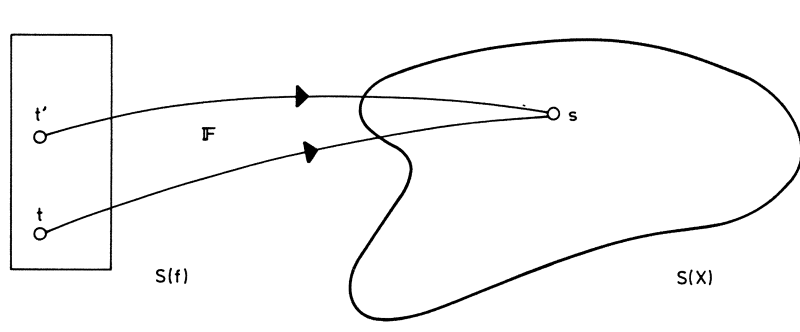
\includegraphics[width=0.6\textwidth]{img/grafico5.18.png}
        \caption{\label{fig:grafico_5_18} Fig. 5.18. [La correspondencia IF: S(j)-'> S(X) de estados de referencia a estados de cosas. IF no tiene por qué
        ser 1-1: dos estados de referencia diferentes pueden corresponder a un único estado de cosa, como en el
        movimiento periódico. Pero IF debe ser sobre: cada estado de cosa debe emparejarse con al menos un
        estado de referencia. ].}
        \end{figure}
    \end{center}
    Las condiciones —independencia y parametrizabilidad— se considerarán
    conjuntamente necesarias y suficientes para caracterizar el concepto general de un
    marco de referencia. (Cada teoría científica puede definir su propio concepto específico
    de marco de referencia añadiendo sus propias condiciones adicionales,
    normalmente que se cumplan ciertas leyes en relación con el marco. Véase Bunge
    (1967b). En resumen, hacemos la
    DEFINICIÓN 5.36 Sea X una cosa representada por el esquema funcional
    Xm = (M, IF) y sea f otra cosa con estados en S(f). Entonces f
    es un marco de referencia para X si y solo si
    (i) f + X es un agregado, de modo que h(f + X) = h(f) u h(X), y
    (ii) el dominio de la función de estado de X es igual al espacio de estados de f,
    es decir, IF: S(f) ~ S(X), de donde M = S(f). 
\end{justifying}